\chapter{工程项目}
\label{ch:concise-engineer}

\begin{introduction}
  \item 了解工程项目的适用场景与向导步骤；
  \item 会设置引脚角色与多套控制模式；
  \item 会用动作行与动作表安排按键动作；
  \item 按架空、低速、逐项的顺序完成实车验证。
\end{introduction}

工程项目用于预制四轮底盘无法覆盖的构型：麦克纳姆轮底盘、全向轮底盘、机械臂，以及
底盘与作业机构组合的机器人。它把控制方式交给使用者安排：先确定每个引脚做什么，再为
每个按键或摇杆安排动作。自由度更高，实车验证也更重要。

\section{适用场景}

表~\ref{tab:concise-engineer-configs} 列出校内赛常见的工程构型与配置要点。运动学关系
不需要手工推导，按动作行逐路安排摇杆与按键即可。

\begin{table}[htbp]
  \centering
  \small
  \begin{tabularx}{\linewidth}{@{}>{\raggedright\arraybackslash}p{0.20\linewidth}
      >{\raggedright\arraybackslash}p{0.30\linewidth}
      >{\raggedright\arraybackslash}X@{}}
    \toprule
    构型 & 特点 & 配置要点 \\
    \midrule
    四轮麦克纳姆轮 & 可前后、左右平移与原地旋转 & 四个轮电机作为独立输出，用动作行把摇杆输入分配到各轮 \\
    三轮全向轮 & 三轮 120 度布置，可全向平移 & 三个轮电机独立输出，按实际安装方位分配 \\
    二自由度机械臂 & 两个舵机，平面内抓放 & 两个舵机端口，配合动作表按档位切换姿态 \\
    底盘与机械臂组合 & 移动与作业合为一体 & 保留预制底盘，另用动作行与动作表控制机械臂 \\
    \bottomrule
  \end{tabularx}
  \caption{常见工程构型与配置要点}
  \label{tab:concise-engineer-configs}
\end{table}

\section{向导步骤}

工程项目向导共七步：遥控器与底盘、PWM 与引脚、模式切换、动作映射、检查与摘要、
生成代码、烧录。

“遥控器与底盘”页与步兵项目相同，但多一个“启用底盘控制”开关。关闭后，四个底盘电机
引脚释放给动作行使用，LX、LY 也可以作为普通输入参与动作（图~\ref{fig:concise-chassis-off}）。
需要自行安排四轮混控时关闭该开关；仍使用标准四轮底盘时保持开启。

\begin{figure}[htbp]
  \centering
  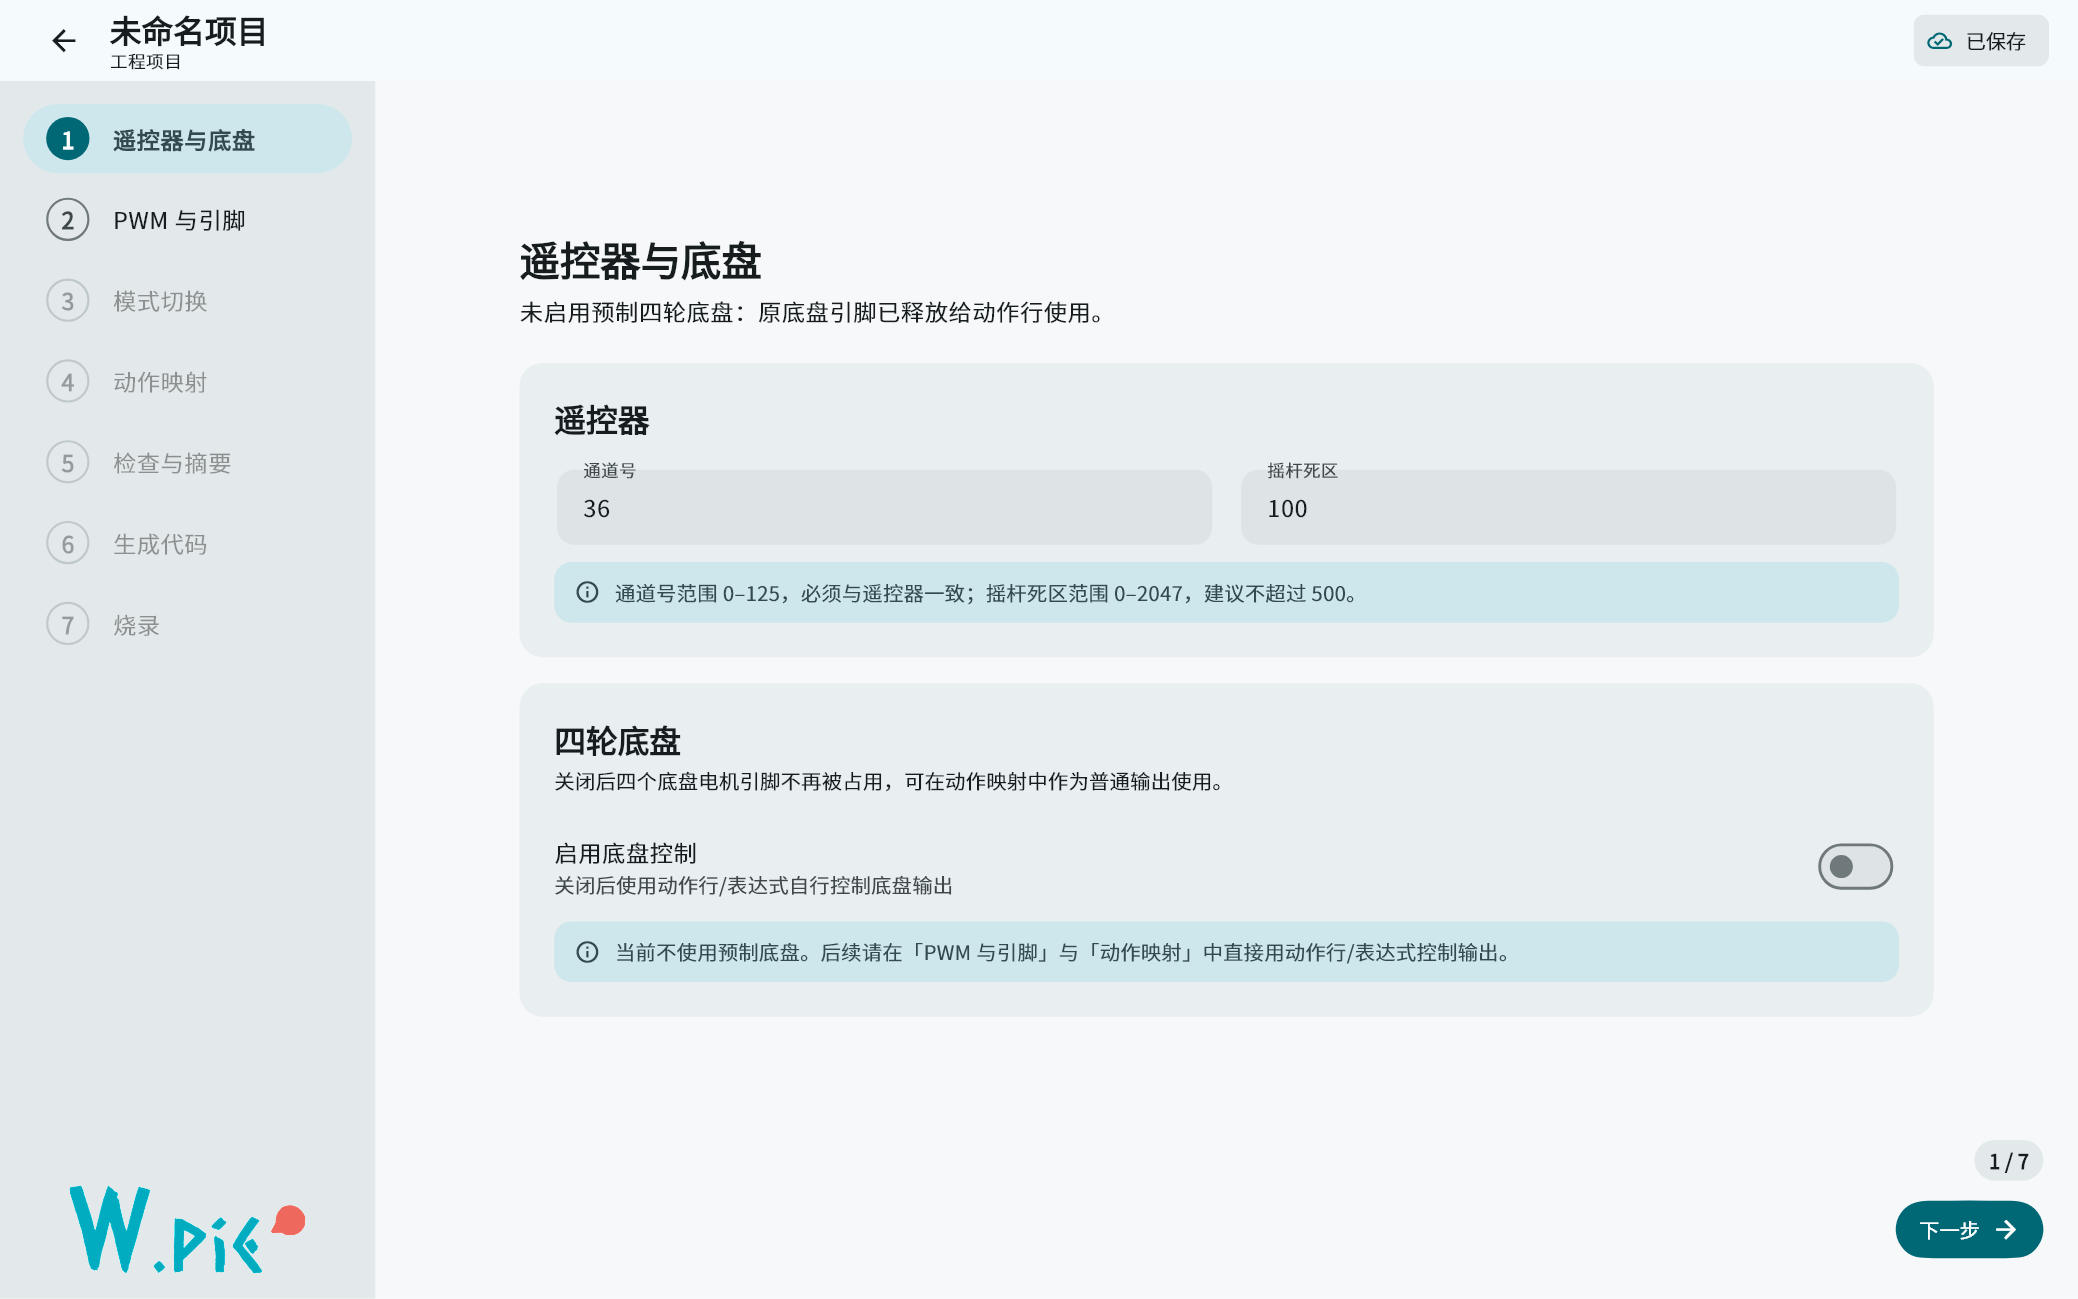
\includegraphics[width=0.95\linewidth]{image/ch05/5-1-chassis-off.png}
  \caption{工程项目关闭预制底盘后的“遥控器与底盘”页：原底盘引脚释放给动作行}
  \label{fig:concise-chassis-off}
\end{figure}

\section{引脚与频率}

“PWM 与引脚”页（图~\ref{fig:concise-pwm}）完成两件事：设置两组引脚的频率，指定每个
引脚的角色。

\begin{figure}[htbp]
  \centering
  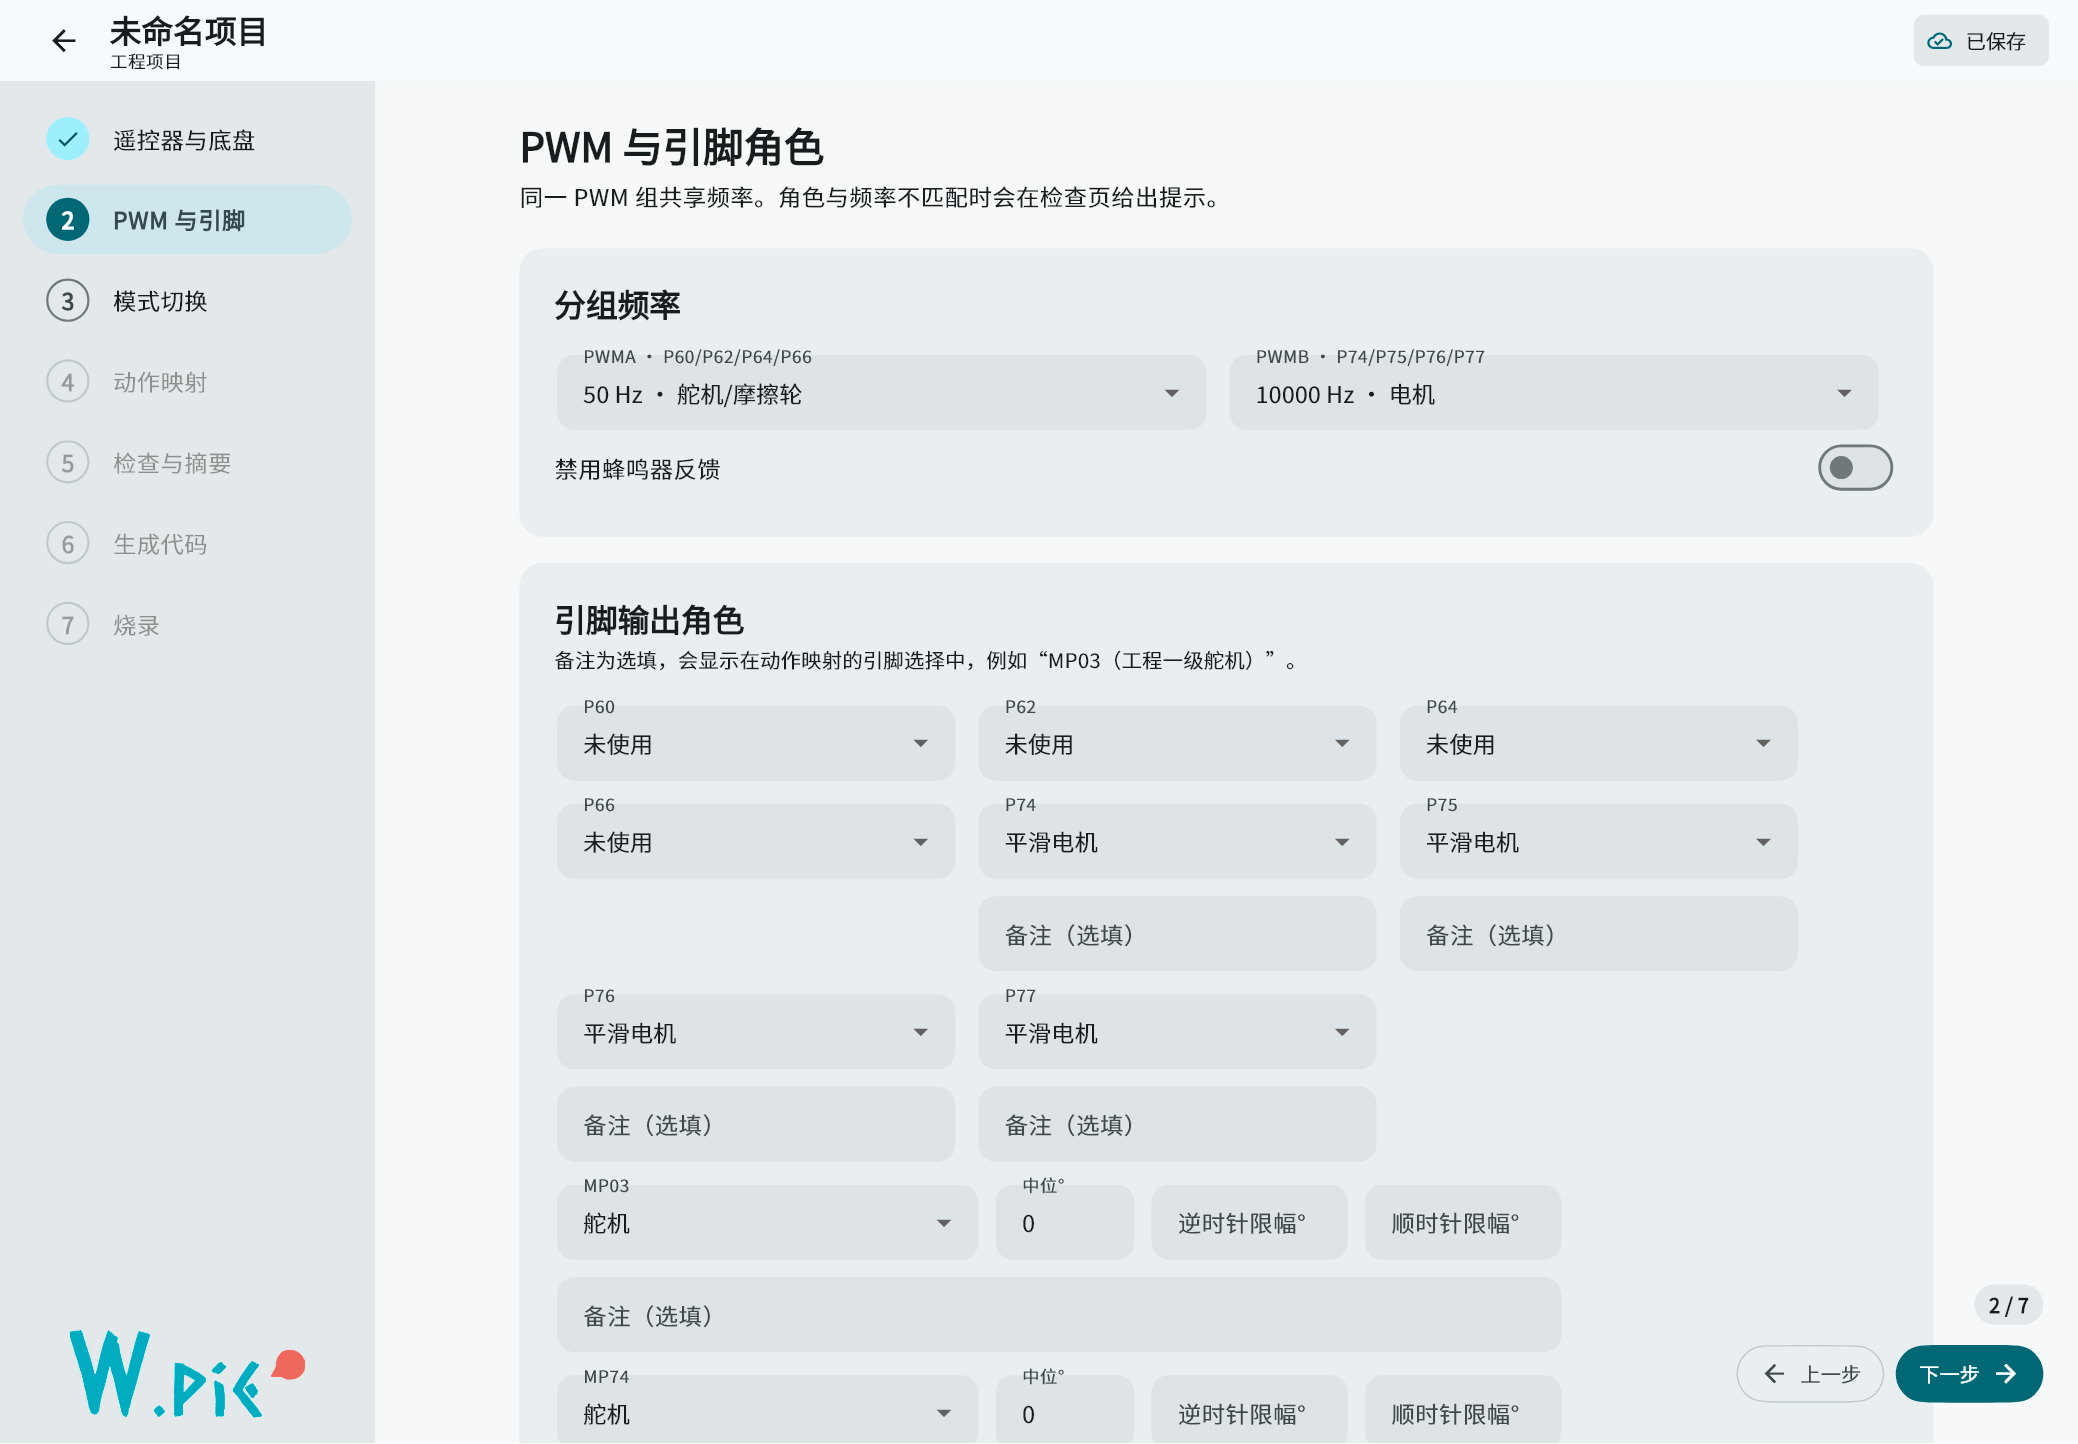
\includegraphics[width=0.95\linewidth]{image/ch05/5-2-pwm-pins.png}
  \caption{“PWM 与引脚”页：分组频率与每个引脚的输出角色}
  \label{fig:concise-pwm}
\end{figure}

同一组内的引脚共享频率：舵机与摩擦轮使用 50\,Hz 组，平滑驱动的电机使用 10000\,Hz 组。
角色与频率不匹配时，检查页会给出提示；不确定时保持默认分组即可。

每个引脚的可用角色由软件按硬件能力限定，下拉框只列出可用项。常用对应关系为：

\begin{itemize}
  \item P60、P62：电机、舵机或摩擦轮；
  \item P74--P77：电机、舵机或摩擦轮；
  \item P64、P66：舵机或摩擦轮；
  \item 主控板 MP03、MP74：舵机或摩擦轮。
\end{itemize}

引脚备注为选填项，只用于在动作行与动作表的下拉框中辨认用途，例如“工程一级舵机”；
备注不参与检查与动作执行。

\section{模式切换}

工程机器人可以设置 1--4 套互相独立的控制映射，用于不同任务。模式数量大于 1 时，需要
选择切换方式：

\begin{itemize}
  \item \textbf{单击轮换}：按同一个切换键，在各模式之间依次轮换；
  \item \textbf{一一对应}：为每个模式指定一个独立按键，按哪个键进入哪个模式。
\end{itemize}

每个模式的动作行与动作表相互独立。切换模式时，未被新模式映射的电机输出会清零，舵机
保持最后位置。因此每个模式都要把该模式需要的输出写全，不能依赖上一个模式的状态。

\section{动作行}

“动作映射”页按模式编辑动作。一个动作行由四部分组成：输入、输出、控制方式与参数。

\begin{itemize}
  \item \textbf{输入}：按键或摇杆轴；不指定输入时，该行只做变量计算；
  \item \textbf{输出}：动作作用的引脚，下拉框只列出已在“PWM 与引脚”页启用的引脚；
  \item \textbf{控制方式}：直接、单次、持续、速度、增速，或摩擦轮的启停、油门单次、
        油门持续、摇杆油门；下拉框只列出该引脚角色支持的方式；
  \item \textbf{参数}：按控制方式填写角度、速度、步长或油门百分比。
\end{itemize}

动作行按列表顺序执行，拖动左侧手柄可以调整顺序。建议一行只安排一个明确动作，先在
架空状态下逐行验证，再组合使用。动作行也支持用变量与表达式组合摇杆输入，用于自定义
混控；该写法不属于本简明版范围，需要时参见完整版教材。

\section{动作表}

动作表用于“一个按键走完一段流程”的机构，例如机械臂抓放、多档位伸缩。与动作行的
区别在于：动作表把一组输出按档位组织成表格，每按一次键前进一档，每个档位是一整列
完整的输出值。

\begin{itemize}
  \item 档位数可设为 2--8 档；
  \item “下一档键”负责前进，可选“上一档键”负责后退；
  \item “越界重复”开启时首尾循环，关闭时到首尾档停住；只有下一档键时固定循环；
  \item 表格按“引脚 × 档位”填写：舵机填带符号角度，电机填带符号速度，摩擦轮引脚
        填油门百分比；
  \item 卡片头部的复制键保留按键、档数与全部单元格，副本插入到源表之后；
  \item 档位较多、超出卡片宽度时，表格下方提供横向滚动条。
\end{itemize}

动作表是“写一次、保持”的控制方式：每档写入后保持，直到下一次按键切换。电机类关节
没有位置反馈，机械臂等机构必须配合机械限位与低速验证，不能只依赖档位数值。

\section{检查与实车验证}

工程项目的检查页会拦住引脚冲突、按键冲突、动作表缺格与越界等问题。由于控制逻辑由
使用者自行安排，检查通过只说明配置自洽，不说明动作符合机械结构，实车验证按以下顺序：

\begin{enumerate}
  \item 车体架空，可能干涉的机构拆下或脱离负载；
  \item 速度、角度、油门都取小值，逐行动作验证方向与幅度；
  \item 确认单个动作正常后，再验证同时输入与模式切换；
  \item 切换模式，确认未映射的电机停止、舵机保持，且没有意外动作；
  \item 全部通过后落地，先低速、空载运行，再逐步增加负载。
\end{enumerate}

\begin{note}
动作表与动作行都可能让机构持续出力。调试时保持手边可随时断电，出现异响、堵转或
超出行程立即切断电源，再回到配置中修改数值。机械限位是最后一道保护，不能省略。
\end{note}
